\documentclass[../main.tex]{subfiles}
\begin{document}

Zur Aufnahme der galaktischen Radiofrequenzen wird das SALSA\footnote{kurz für: \textit{Such A Lovely Small Antenna}}-Onsala Teleskop genutzt. Dieses steht im \textit{Onsala Space Observatory} in Schweden und kann aus der Ferne kontrolliert werden\footnote{https://brage.oso.chalmers.se/salsa/welcome}. Das Teleskop ist für die Frequenz \SI{1420}{\mega\hertz} optimiert, die mit der Emissionsfrequenz der Hydrogengaswolken gut übereinstimmt. Die Frequenzauflösung von SALSA kann manuell eingestellt werden, die beugungsbedingte Winkelauflösung beträgt nach dem FWHM-Kriterium etwa \SI{5.4}{\degree}.\\ 

\noindent Zur Orientierung des Teleskops stehen für diesen Versuch zwei relevante Koordinatensysteme zur Verfügung: das der Sonne und das galaktische System. Bei ersterem liegt die Sonne im Zentrum, Abweichungen von ihrer Position werden durch einen Höhenwinkel $l$ und einen Azimutwinkel $a$ angegeben. Das Teleksop hat die Fähigkeit, die Sonne um einen gegebenen Offset $(l,a)$ automatisch zu verfolgen. Unsicherheiten bei diesem Verfolgen sind dabei vernachlässigbar klein gegenüber der Winkelauflösung.

 Für das Hauptziel des Versuchs, die Beobachtung der Milchstraße, dient das galaktische System. Der Erdhimmel wird hier durch eine galaktische Länge $l$ und eine galaktische Breite $b$ kartographiert. Wie diese beiden krummlinigen Achsen festgelegt sind, ist in Abbildung skizziert.
\begin{figure}[H]
    \centering
    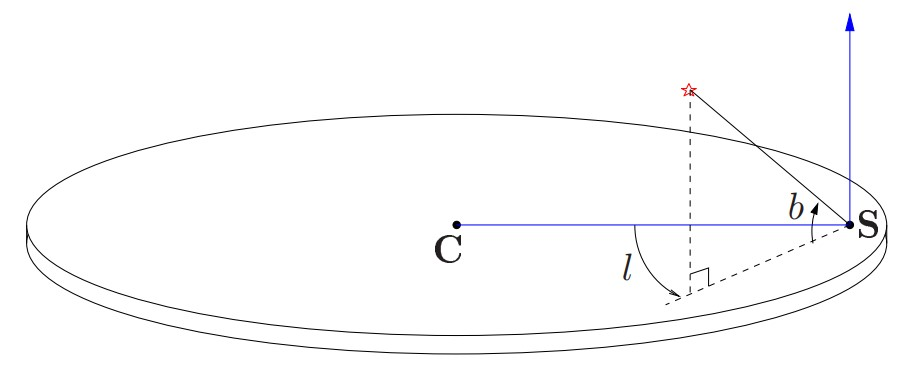
\includegraphics[width=7cm]{Bilddateien/Aufbau/GalaktischesSystem.jpg}
    \caption{Festlegung des galaktischen Koordinatensystems: Die Verbindungslinie zwischen des Sonnensystems (S) und des Galaxiezentrums (C) markiert den Ursprung $l=\SI{0}{\degree}$ und $b=\SI{0}{\degree}$. Innerhalb der galaktischen Scheibe wird gegen den Uhrzeigersinn die galaktische Länge $l$ erhöht. Dahingegen werden Blickwinkel aus der galaktischen Scheibe heraus mit dem Breitengrad $b$ gemessen.}
\end{figure}

\noindent Abbilddung \ref{fig:AufbauSteuerpult} zeigt das digitale Steuerungspult des Teleskops, in dem sich die komplette Versuchsdurchführung abspielt.  
\begin{figure}[H]
    \centering
    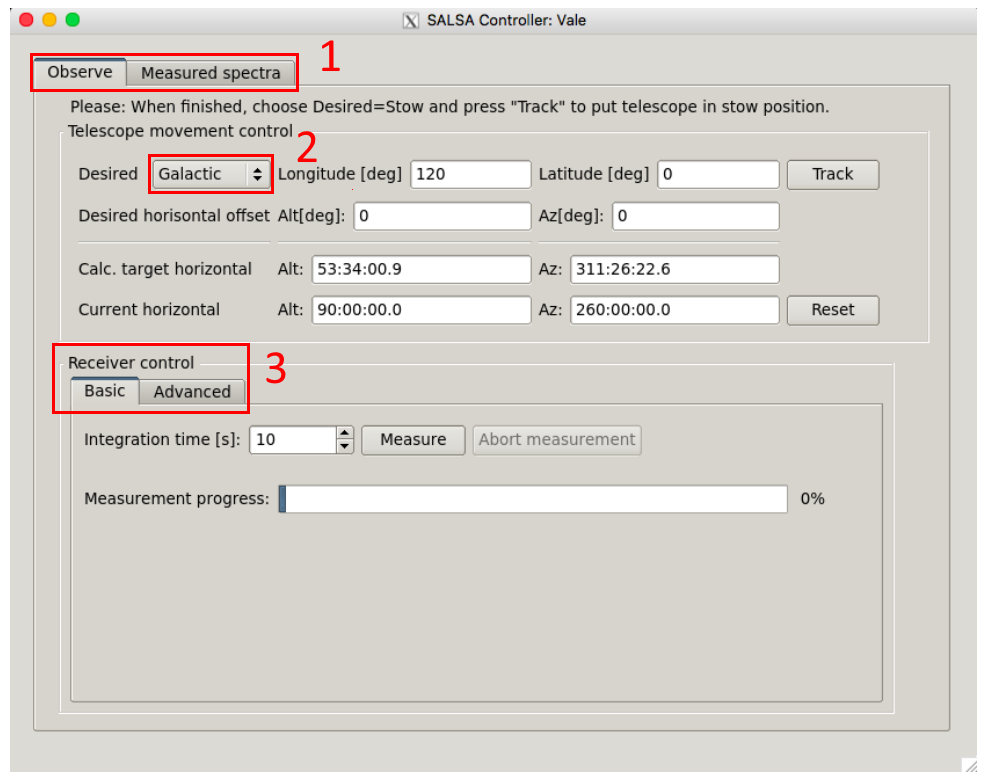
\includegraphics[width=12cm]{Bilddateien/Aufbau/AufbauSteuerpult.png}
    \caption{Steuerpult des SALSA-Onsala Teleskops. Im Bereich \textcolor{red}{(1)} lässt sich wählen zwischen der Steuerung des Teleskops und der Anzeige von aufgenommenen Daten. Das gewünschte Koordinatensystem (Sonne, galaktisch) kann in der Auswahl \textcolor{red}{(2)} eingestellt werden, daneben werden die entsprechenden Koordinaten eingetragen. Darunter kann der Offset für diese Koordinaten eingetragen werden, beim Drücken des \glqq{}track\grqq{}-Knopfes stellt sich das Teleskop dann auf die eingewählten Koordinaten plus den Offset ein. Im Bereich \glqq{}receiver control\grqq{} kann unter dem Reiter \glqq{}basic\grqq{} die Integrationszeit für aufgenommenen Spektren eingestellt werden, also über welchen Zeitraum die Daten gemittelt werden sollen. Unter dem Reiter \glqq{}Advanced\grqq{} lässt sich einstellen, in welchen Frequenzbereich messen soll sowie den Modus der Messung. Der \glqq{}switched\grqq{}-Modus dient zur spektralen Aufnahme, der \glqq{}signal\grqq{}-Modus zur Messung der totalen empfangenen Leistung.}
    \label{fig:AufbauSteuerpult}
\end{figure}
        
\end{document}